
\chapter{Introduction}
\label{chap:wifi-cam}

% \section*{Introduction}
% \label{sec:cam-intro}

Personal wireless surveillance cameras are affordable nowadays.
From the hotel receptions to the home surveillance, many reason can justify the usage of a video camera.
While these cameras have valid usages, it is an open door to very important privacy threats.
During the placing of this kind of personal cameras, the question of security is often neglected or completely forgotten.\\

This chapter describes the different types of cameras and the choice of case study.
The wireless cameras are divided in two types: analogical and digital cameras.

\section{Analogical cameras}
\label{sec:cam-analogic}

Analogical video cameras are often cheaper than the digital models, which explains the fact they are still in use nowadays.
The video camera records analogical pictures and transmits it on a defined radio frequency.
To visualise the video, a receptor is set on the same frequency.
The frequency bands used are usually around 2,4GHz and have been selected as to avoid conflict with other emissions.\\

The important aspect about these camera is the fact that, as the video is broadcasted on a defined frequency, any receptor set on this frequency can receive and watch the video stream.
This implies that there is technically no protection on the video stream.
Anybody using a portable receptor is able to watch the video stream (which could also contain an audio stream depending on the camera model) at a range of a few metres.\\

The usage of this type of camera should only be reserved for non sensible content and be considered as watchable by anybody.

\section{Digital cameras}
\label{sec:cam-digital}

Unlike the analogical video cameras, the digital models record digital images and transmit it using numerical stream, in this case, using wifi networks.
The protection of the video stream is then possible at several level:\\

\begin{itemize}
\item Encryption of the wireless network (WEP, WPA, WPA2...)
\item Encryption of the transmission protocol (usage of SSL to transmit the images)
\item Access control mechanism to the stream itself (password to access the admin interface)
\end{itemize}

The choice of security mechanism is then directly related to the security of the video stream.
Using weak security mechanism (for example WEP) leads to a weak security of the camera.\\

The digital video cameras can contain many features for the transmission of the video stream.
As these features improve the convenience by allowing users to access in several different ways (admin interface, mail sending...), all these methods are not equals in term of security.
This difference is often unknown and confuses the end user in an incorrect sense of security (eg: setting an admin password to the administration interface during the configuration process does not protect the RTSP\footnote{RTSP, for \emph{Real Time Streaming Protocol}, is a streaming protocol, often used to embed the video stream in third parties softwares.} stream in the analysed D-Link camera).

\section{Web cameras}
\label{sec:cam-google}

To be able to watch the video stream of the camera from any machine connected to the Internet, some users configure their cameras to be accessible from the outside of the home network.
If these digital cameras are not protected with an access control mechanism, anybody with the correct address can watch it.
Often the owners of such cameras rely on the fact that these cameras are not published or accessed by a very small number of authorised people.
However it is possible to find and access the video stream of such cameras in some cases.

\subsection{Google searches}
\label{sec:cam-google}

In some cases, the cameras streams are published on websites for the usage of concerned public.
This can be the case for streets or parking cameras in neighbour or school associations for example.
As the cameras are accessible on the Internet, it may be detected and indexed by a search bot software such as the ones Google uses to constitute his search engine.
If indexed, these cameras can be listed with the correct search keywords.\\

Using the Google search engine, the keyword \texttt{inurl:} is used to search in the site's URL itself.
On certain models of digital cameras, the URL to access the web interface contains some patterns typical of these cameras.
It is the case for example of \texttt{axis-cgi/mjpg} or \texttt{ViewerFrame?Mode=} that are present mostly in webcam server softwares.
Using the following search queries can list links to these cameras:

\begin{itemize}
\item \texttt{inurl:ViewerFrame?Mode=}
\item \texttt{inurl:ViewerFrame?Mode=Refresh}
\item \texttt{inurl:axis-cgi/jpg}
\item \texttt{inurl:axis-cgi/mjpg}
\item \texttt{inurl:view/indexFrame.shtml}
\item \texttt{inurl:view/index.shtml}
\item \texttt{inurl:view/view.shtml}
\end{itemize}

While these cameras are, most of the time, filming public areas that were already publicly available, these search queries allow quickly to list a large quantity of cameras.
By refining the search with other keywords such as \emph{airport} or the name of cities, it may make easier the collect and cross-checking information and facilitate abuses.\\

Also some personal cameras were not meant to be mentioned on websites, it is possible with basic programming knowledge to create programs scanning a defined range of IP addresses to detect the one responding to the search URL pattern.
A similar script has been developed to detect the model of D-Link cameras studied in Chapter \ref{chap:cam-dcs}.\\

While some cameras found by searches are protected, some are wrongly configured and still use default settings such the default administrator account's credentials for example (which can be found easily in user manuals).
In such cases, the full control and configuration of the camera would be accessible to a distant attacker.

\subsection{TRENDnet vulnerability}
\label{sec:trendnet-hack}

While the methods mentioned previously abuse from a lack of protection, some cameras, even protected, suffer from vulnerabilities and the video stream can be accessed if they are published on the web.
This is the case of a set of TRENDnet IP cameras on which a bug has been discovered.\\

In January 2012, the author of the webblog Console Cowboys, has published some researches he made about an TRENDnet digital camera~\cite{trendnet-hack}.
Through his researches, he discovered a executable binary that with access rights open to any user, even unauthenticated.
From these conclusion, he concluded that using the URI \texttt{/anony/mjpg.cgi} on any camera using this firmware reveals the video stream of the camera as shown in Figure \ref{fig:trendnet-hack}.\\

\begin{figure}[h]
  \centering
  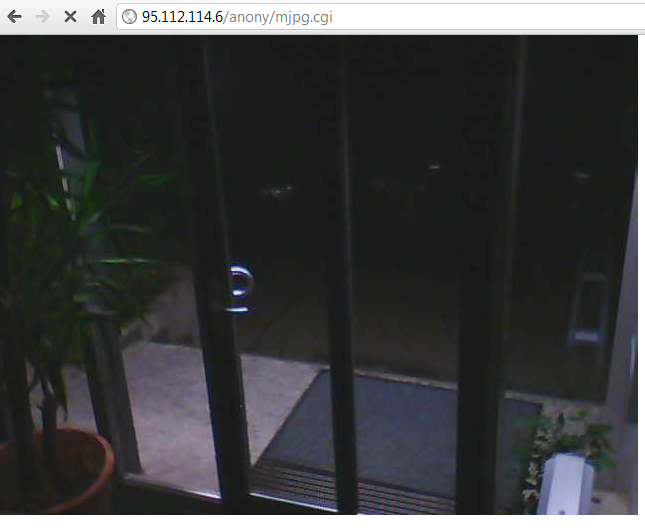
\includegraphics[width=7cm]{images/trendnet-hack.png}
  \caption{Example of video stream accessed on a vulnerable camera}
  \label{fig:trendnet-hack}
\end{figure}

The exploitation of this vulnerability is made easier by the existence of ShodanHQ\footnote{SHODAN - Computer Search Engine \url{http://shodanhq.com/}}, a search engine targeted at the indexing of IP devices.
Using the query \texttt{netcam} which is used in the headers of any TRENDnet camera, the search engine lists IP addresses of cameras publicly available from an IP address and on which the vulnerability can be tested.\\

TRENDnet replied to this publication by proposing an update of the firmware that fixes the vulnerability.
However, the proportion of vulnerable cameras may stay large for a long time as cameras are very unlikely to be updated by the owners of such devices.\\

This vulnerability is an example of the danger of setting up such devices on the web.
Even by protecting correctly and not publishing the URL to access the camera, owners of these devices are vulnerable to any curious eyes if they allow the access from the outside of their network.
Unlike the results from the Google Search in Section \ref{sec:cam-google}, these cameras are often personal cameras and are often used in private areas.
A similar bug permitting the access to the log file on the studied camera has been discovered is explained in Section \ref{sec:dcs-log}.